\scanpage{39}
\mspage{20}
repère \inserted{les} $u(\widetilde a_i^\omega)$, résulte déjà de celle de $\xi$, qui repère \inserted{les} $u(d_i^\omega)$,
\figure{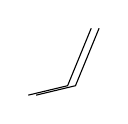
\begin{tikzpicture}[baseline=0pt]\draw (0,0)--(.5,.12)--(.8,.85);\draw (.1,0)--(.6,.12)--(.9,.85);\end{tikzpicture}}
Les graphes $\mathrm{I}$ à $\mathrm{VII}$ donnent lieu au diagramme d'inclusions
\diagram{\begin{tikzcd}[ampersand replacement=\&,column sep=2em,row sep=2.8em,execute at end picture={\draw ([xshift=-4mm,yshift=5mm]\tikzcdmatrixname-2-1.north west) rectangle ([xshift=5mm,yshift=-4mm]\tikzcdmatrixname-3-3.south east);}]
\&\&\mathrm{III}\arrow[dl,hook]\arrow[dr,hook]\&\&\\
\mathrm{I}\arrow[r,hook]\arrow[dr,hook]\&\mathrm{II}\arrow[dr,hook]\arrow[r,draw=none,"\unsure{\deleted{\leftrightarrow}|\leftrightarrow}"]\&\phantom{\mathrm{II}}\&\mathrm{IV}\arrow[dl,hook]\&\mathrm{V}\arrow[l,hook]\\
\&\mathrm{VII}\arrow[r,hook]\&\mathrm{VI}\&\&
\end{tikzcd}}\quad(68)

Sans calcul, je peux déjà prédire que la donnée d'un autom. de $\mathrm{VII}$ fixant les sommets et commutant à $\unsure{\mathcal G_J|G_J}$, équivaut à la donnée des quantités
\[
(69)\qquad (\uline{\lambda},\beta',\uline{\xi'})\in\widehat\Pi_{0,3}\times\widehat\Pi_{0,3}\times\widehat\Pi_{0,3}
\]
reliés par \deleted{\unsure{les}} \unsure{l'|les} équations \deleted{(63) ici}
\[
(70)\qquad\left\{\begin{aligned}
\beta'&=\alpha'\sigma_\infty(\lambda)\\
\beta'\sigma_\infty(\beta')&=1
\end{aligned}\right.\qquad
\begin{gathered}
\text{où}\quad\alpha'=\xi'\rho^{\unsure{\phantom{-1}|-1}}(\xi')^{-1}\\
\text{i.e.}\quad\alpha'\sigma_\infty(\lambda)\sigma_\infty(\alpha')\lambda=1
\end{gathered}
\]
\margin{\figure{
\begin{tikzpicture}\node[align=center] at (0,.6) {donc $\beta'$\\inutile!};\draw (-.8,.6)..controls (-.9,-.1) and (-.2,-.3)..(0,-.6)..controls (.05,-.1) and (.85,-.2)..(.9,.35);\end{tikzpicture}}}
(\unsure{tout|tandis} comme \inserted{dans le cas où} $\mathrm{II}$ est défini par \deleted{$(\lambda,\eta,\alpha')$},
\deleted{reliés par}
\[
(69')\qquad(\uline{\lambda},\uline{\eta},\alpha')\in\widehat\Pi_{0,3}\times\widehat\Pi_{0,3}\times\widehat\Pi_{0,3}
\]
avec \unsure{l'|les} équations
\[
(70')\qquad\left\{\begin{aligned}
\beta'&=\alpha'\sigma_\infty(\lambda)\\
\alpha'\rho(\alpha')\rho^2(\alpha')&=1
\end{aligned}\right.\qquad\text{où}\quad\beta'=\eta\sigma_\infty(\eta)^{-1}
\]
\margin{donc $\alpha'$ inutile!}
\margin{38}
